\section{Timing}\label{sec:timing}
\subsection{Profiling}
In order to find the bottleneck of the code, we first profiled
 timing of each steps using Intel’s VTune Amplifier. See Listing~\ref{lst:amplxe_command}.

\begin{lstlisting}[caption={VTune Amplifier Command},label={lst:amplxe_command},frame=single,language=bash]
amplxe-cl -collect advanced-hotspots ./shallow
amplxe-cl -report hotspots -source-object function=<NAME>

amplxe-cl -report hotspots -r r001ah/ > all
amplxe-cl -report hotspots -source-object function="Central2D
<Shallow2D, MinMod<float>>::compute_step" > compute_step
\end{lstlisting}

\subsection{Initial Profile Result}

From the Listing~\ref{lst:initial_profile_result}, we could figure out "limited\_derivs", "compute\_step", and "compute\_fg\_sppeds" take longest time (See profile.sh code). Among these results, "limited\_derivs" function definitely was the worst bottleneck.

\begin{lstlisting}[caption={Initial Profile Result},label={lst:initial_profile_result},frame=single,language=bash]
Function                     Module        CPU Time
-----------------------------------------  --------
limited_derivs               shallow         1.378s
compute_step                 shallow         0.640s
compute_fg_speeds            shallow         0.219s
_IO_fwrite                   libc-2.12.so    0.019s
_IO_file_xsputn              libc-2.12.so    0.015s
[Outside any known module]   [Unknown]       0.014s
run                          shallow         0.006s
write_frame                  shallow         0.006s
solution_check               shallow         0.004s
offset                       shallow         0.002s
do_lookup_x                  ld-2.12.so      0.001s
operator[]                   shallow         0.001s
\end{lstlisting}

\subsection{Initial Timing Result}
We made simple script to generate timing plots (See plotter.sh code). Here, x-axis indicates the number of cells per side. We swept this from 100 to 500. Y-axis shows the number of cells per side per average time, which means cell per seconds. We divided timing by the cube of nx. Also, another graph simply shows that timing vs. nx. 

Initial timing result can be found at Figure ~\ref{fig:initial_timing_result1} and Figure ~\ref{fig:initial_timing_result2} .

\begin{figure}[h]
    \centering
    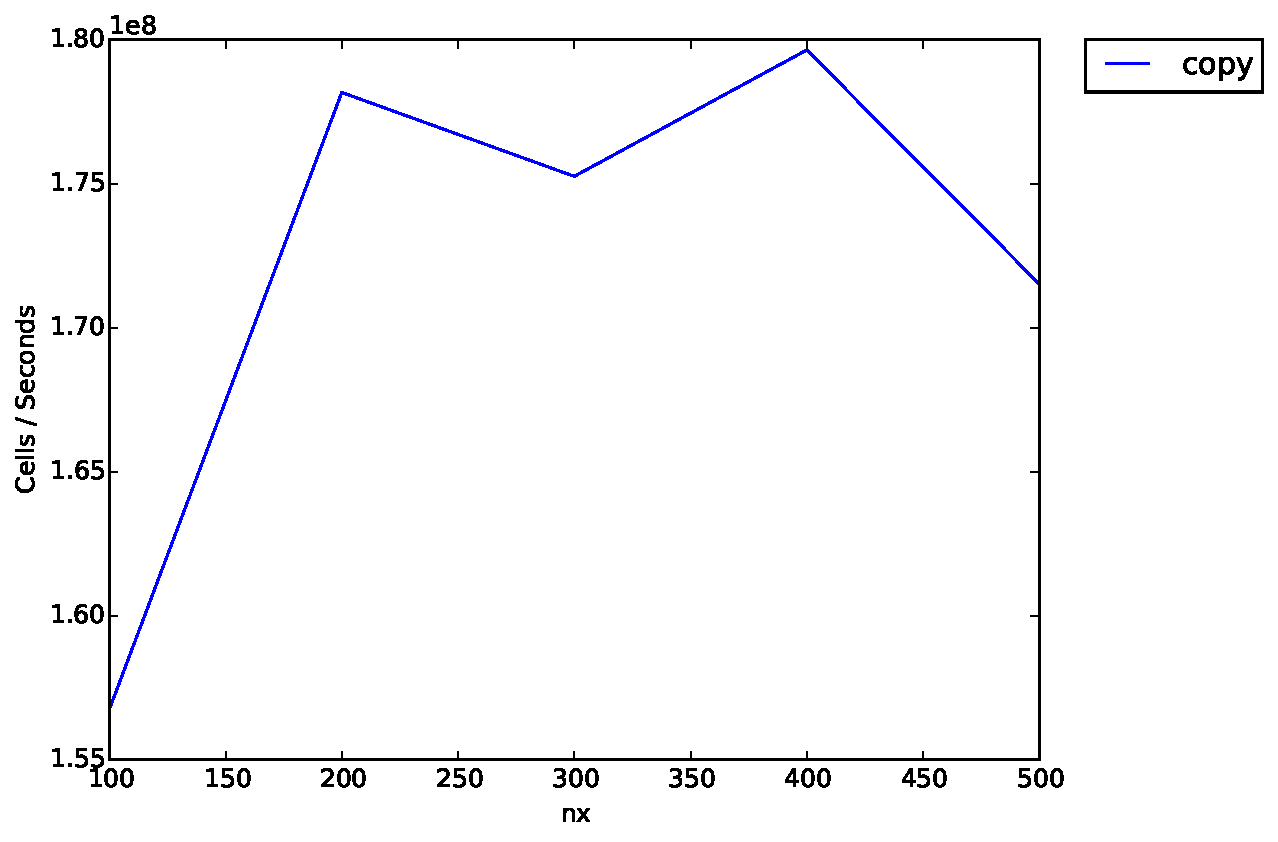
\includegraphics[width=0.8\textwidth]{figs/init-timing1.pdf}
    \caption{Initial Timing Result (cells/seconds vs. nx)}
    \label{fig:initial_timing_result1}
\end{figure}

\begin{figure}[h]
    \centering
    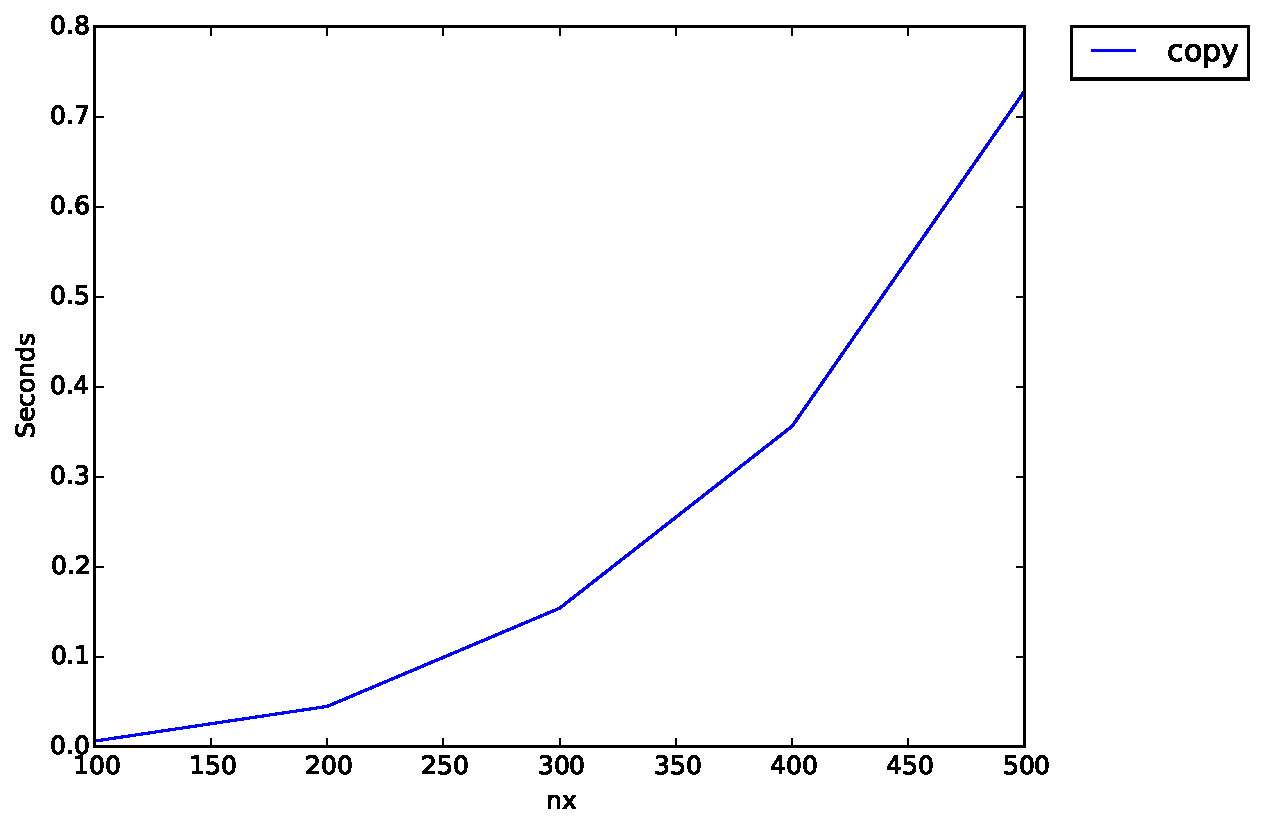
\includegraphics[width=0.8\textwidth]{figs/init-timing2.pdf}
    \caption{Initial Timing Result (seconds vs. nx)}
    \label{fig:initial_timing_result2}
\end{figure}